% !TeX root = prob.tex

\section{Random Walk}\label{s.walk}

\textbf{Problem} A particle is placed at the origin of the $x$-axis. It repeatedly takes steps: right with probability $p$ and left with probability $q=1-p$.
\begin{enumerate}
\item What is the probability that the particle will return to the origin?
\item What is the expected duration until the particle returns to the origin?
\end{enumerate}
\begin{center}
\begin{tikzpicture}[scale=1.2]
\draw[<->] (-6,0) -- (6,0);
\foreach \x in {-5,-4,-3,-2,-1,0,1,2,3,4,5} {
  \draw (\x,0) -- +(0,4pt);
  \node at (\x,-10pt) { $\x$ };
}
\node at (-6,-10pt) { $\cdots$ };
\node at (6,-10pt) { $\cdots$ };
\draw[fill] (0,7mm) circle[radius=1pt];
\draw[->] (0,7mm) -- node[above] {$q$} +(-1,0);
\draw[->] (0,7mm) -- node[above] {$p$} +(1,0);
\end{tikzpicture}
\end{center}
The clearest presentation of one-dimensional random walk is in \cite{border}, but the derivation of the expected duration is in \cite{privault}.

\subsection{Theoretical results}

By symmetry let the first step be to the right.\footnote{This is equivalent to a first step to the left if $p$ and $q$ are exchanged.} The particle can only return to the origin after an even number of steps. Assume that $p=1/2$. Let $S_{2m}$ be the position of the particle after $2m$ steps. Then:
\[
P(S_{2m}=0) = \dischoose{2m}{m}\disfrac{1}{2^{2m}}\,,
\]
which by Stirling's formula is:
\[
P(S_{2m}=0) \approx \disfrac{1}{\sqrt{\pi m}}\,.
\]
It can now be proved that the probability of a return to the origin is $1$.

For $p\leq 1/2$, $P_{\mathit{origin}}$, the probability of a return to the origin, is $1$ and for $p\geq 1/2$ the probability is (Figure~\ref{f.walk1}):
\[
P_{\mathit{origin}} = \disfrac{q}{p}=\disfrac{1-p}{p}\,.
\]
\begin{figure}
\begin{center}
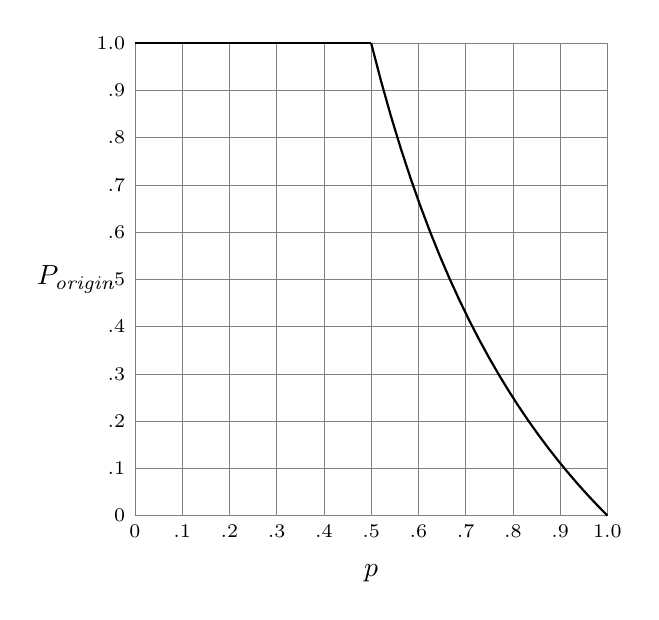
\begin{tikzpicture}[scale=6]
\draw[help lines,step=.1] (0,0) grid (1,1);
\foreach \x in {0,.1,.2,.3,.4,.5,.6,.7,.8,.9,1.0}
  \node[below] at (\x,0) {$\scriptstyle \x$};
\foreach \y in {0,.1,.2,.3,.4,.5,.6,.7,.8,.9,1.0}
  \node[left] at (0,\y) {$\scriptstyle \y$};
\draw[domain=0:.5,thick] plot (\x,1);
\draw[domain=.5:1,thick] plot (\x,{(1-\x)/\x});
\node at (.5,-3.5pt) {$p$};
\node at (-3.5pt,.5) {$P_{\mathit{origin}}$};
\end{tikzpicture}
\caption{Graph of $P_{\mathit{origin}}$}\label{f.walk1}
\end{center}
\end{figure}

$E_{\mathit{origin}}$, the expected duration until the first return to the origin, is infinite for $p\geq 1/2$ while for $p<1/2$ it is:
\[
E_{\mathit{origin}}=\disfrac{1}{q-p}=\disfrac{1}{1-2p}\,.
\]

\subsection{Program structure}

\verb+configuration.py+ contains declarations of variables which are intended to be constant.

\verb+random_walk_plot.py+ contains the functions for plotting a graph of the proportion of simulations that return to the origin and the mean durations if the simulation is run for multiple probabilities or limits.

\verb+random_walk.py+ is the main program which obtains the parameters, runs the simulations, prints the output and calls the plotting functions.

\subsection{Running the simulations}

The program asking the user how to run the simulations and then runs them in a loop. You can run the same simulation again with the saved parameters, enter new parameters, or run a sequence of simulations for a range of probabilities or limits. A typical output is:
\begin{verbatim}
Probability = 0.50, step limit   = 1000
Proportion returning to origin   = 0.977
Probability of return to origin  = 1.000
Proportion reaching limit        = 0.023
Mean duration (steps)            = 49
Expected duration (steps)        = infinity
\end{verbatim}
The proportion of wins in the simulation are very close to the theoretical probability, but the mean duration is far from infinite because the step limit was too small.  The proportion of wins and the mean durations are shown in Figures~\ref{f.random-walk-01} and \ref{f.random-walk-02}.
\begin{figure}
\begin{center}
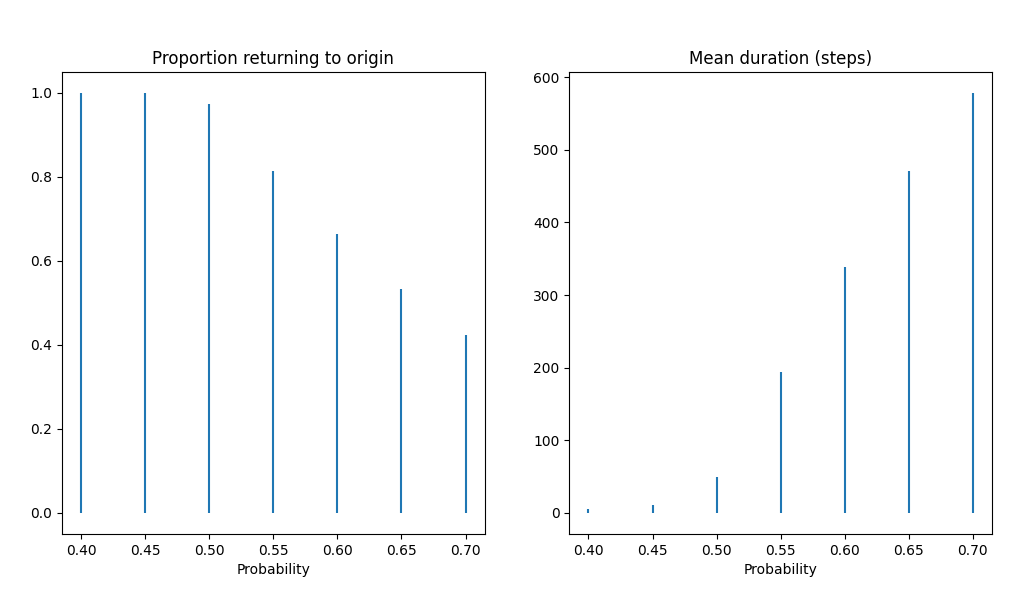
\includegraphics[width=\textwidth]{random-walk-01}
\caption{Proportion of returns to origin and and mean durations for multiple probabilities}\label{f.random-walk-01}
\end{center}
\end{figure}
\begin{figure}
\begin{center}
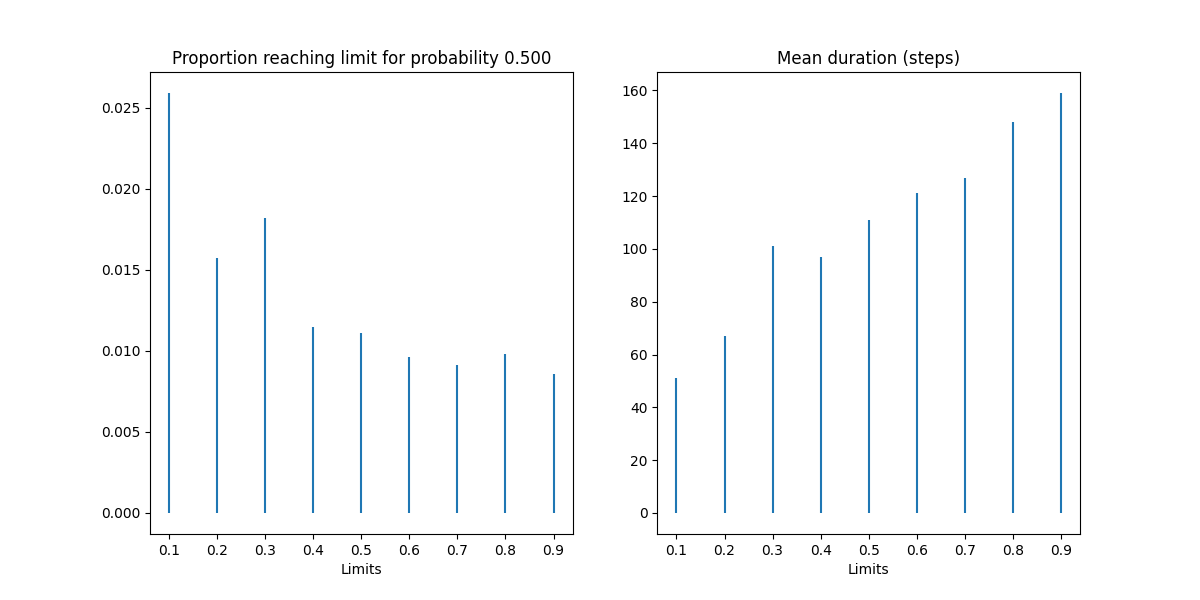
\includegraphics[width=\textwidth]{random-walk-02}
\caption{Proportion of returns to origin and mean durations for multiple limits}\label{f.random-walk-02}
\end{center}
\end{figure}

\subsection{Two-dimensional random walk}

In a two-dimensional random walk a step of the particle consists of one step left or right on the $x$-axis with probability $1/2$ and simultaneously one step up or down on the $y$-axis also with probability $1/2$ (Figure~\ref{f.2d-random-walk}).

\begin{figure}
\begin{center}
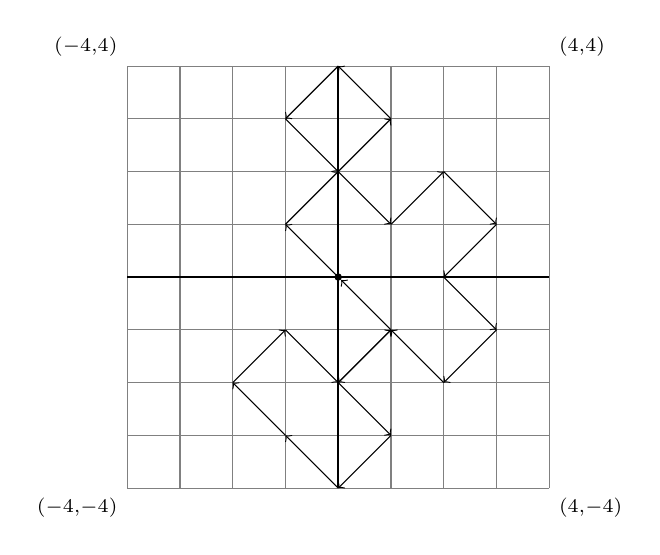
\begin{tikzpicture}[scale=.67]
\draw[color=gray] (-4,-4) grid (4,4);
\draw[thick] (-4,0) -- (4,0);
\draw[thick] (0,-4) -- (0,4);
\node[below left] at (-4,-4) {$\scriptstyle (-4,-4)$};
\node[below right] at (4,-4) {$\scriptstyle (4,-4)$};
\node[above left] at (-4,4) {$\scriptstyle (-4,4)$};
\node[above right] at (4,4) {$\scriptstyle (4,4)$};
\fill (0,0) circle[radius=2pt];
\draw[->] (0,0)  -- (-1,1);
\draw[->] (-1,1) -- (0,2);
\draw[->] (0,2)  -- (1,3);
\draw[->] (1,3)  -- (0,4);
\draw[->] (0,4)  -- (-1,3);
\draw[->] (-1,3) -- (0,2);
\draw[->] (0,2)  -- (1,1);
\draw[->] (1,1)  -- (2,2);
\draw[->] (2,2)  -- (3,1);
\draw[->] (3,1)  -- (2,0);
\draw[->] (2,0)  -- (3,-1);
\draw[->] (3,-1) -- (2,-2);
\draw[->] (2,-2) -- (1,-1);
\draw[->] (1,-1) -- (0,-2);
\draw[->] (0,-2) -- (1,-3);
\draw[->] (1,-3) -- (0,-4);
\draw[->] (0,-4) -- (-1,-3);
\draw[->] (-1,-3)-- (-2,-2);
\draw[->] (-2,-2)-- (-1,-1);
\draw[->] (-1,-1)-- (0,-2);
\draw[->] (0,-2) -- (1,-1);
\draw[->] (1,-1) -- (.055,-.055);
\end{tikzpicture}
\end{center}
\caption{A $22$-step two-dimensional random walk}\label{f.2d-random-walk}
\end{figure}
The probability $1$ the particle will return to the origin but the expected duration is infinite! Therefore, when you run the simulation with any reasonable limit on the number of steps, the proportion of returns to the origin will be much less than $1$ and the mean duration will be quite large:
\begin{verbatim}
Limit                            = 100000
Proportion returning to origin   = 0.777
Proportion reaching limit        = 0.223
Mean duration (steps)            = 24133
\end{verbatim}

The program structure is the same as for the one-dimensional random walk. You can enter the step limit parameter for each simulation interactively and can run the simulations for a range of limits expressed as percentages of the parameter. Figure~\ref{f.random-walk-2D} shows the proportion of returns to the origin and the mean durations for a range of limits.

\begin{figure}
\begin{center}
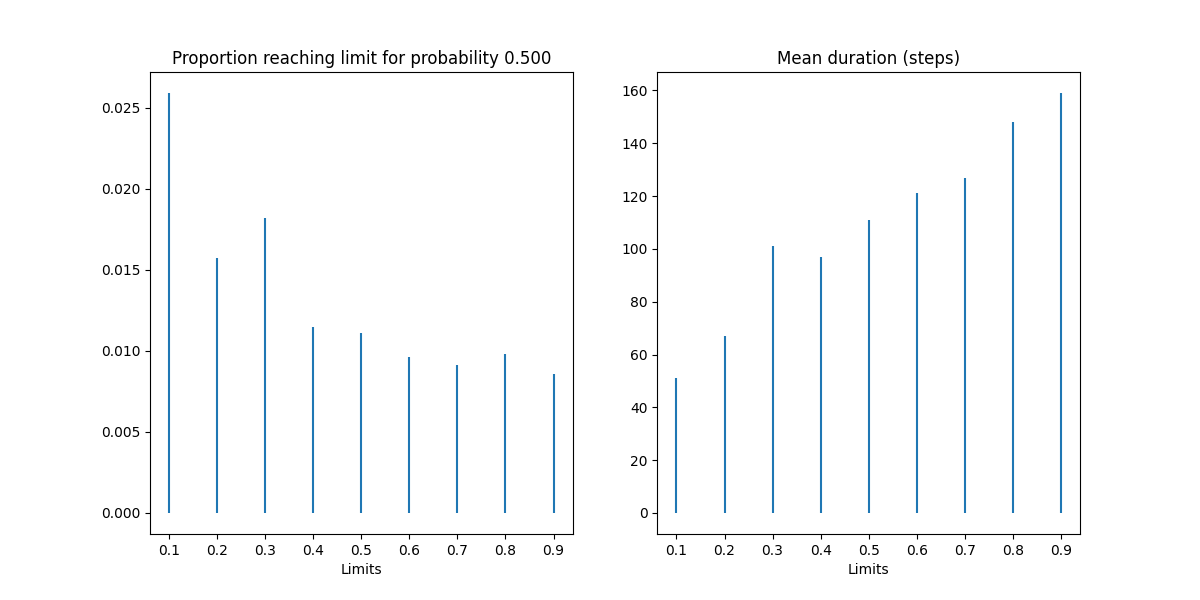
\includegraphics[width=\textwidth]{random-walk-02}
\caption{Proportion of returns to origin and and mean durations for multiple limits}\label{f.random-walk-2D}
\end{center}
\end{figure}
